\chapter{Hexagonales Schach}

Hexagonales Schach hat viele unterschiedliche Spielweisen. Diese variieren nicht nur in den möglichen Zügen, sondern auch der Anzahl der Spielsteine und der Größe des Spielfelds. Glinskis Regeln werden für die Europameisterschaften in hexagonales Schach genutzt \cite{Gados:Hexagonal}. In der Version von Glinski besteht das Spielbrett aus 91 Feldern. Da jede Seite gleichlang ist, ist das Feld ein perfektes Hexagon. Dies ist nicht in jeder Schachvariante gleich. Schafran lässt die Spalten a und l aus (vgl. Abbildung \ref{fig:hex:start}). Dazu variiert noch die Startaufstellung.

\begin{figure}[H]
    \centering
    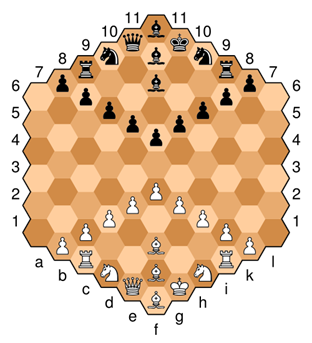
\includegraphics{images/hexStart.png}
    \caption{Startaufstellung Glinski \protect\footnotemark}
    \label{fig:hex:start}
\end{figure}
\footnotetext{\url{https://commons.wikimedia.org/wiki/Category:Glinski\%27s_hexagonal_chess}}

\begin{table}
    \centering
    \begin{tabular}{|c|c|}
        \hline
        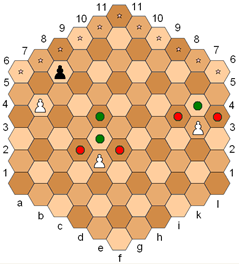
\includegraphics{images/hexPawn.png} & 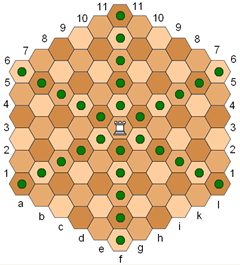
\includegraphics{images/hexRook.png} \\ \hline 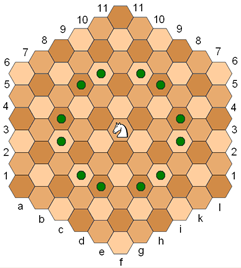
\includegraphics{images/hexKnight.png} & 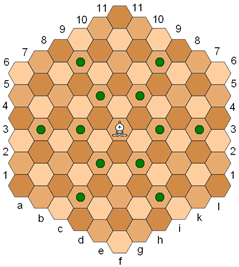
\includegraphics{images/hexBishop.png} \\ \hline 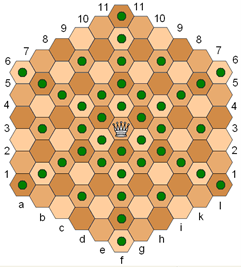
\includegraphics{images/hexQueen.png} & 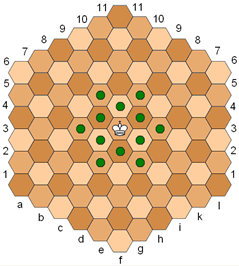
\includegraphics{images/hexKing.png} \\ \hline
    \end{tabular}
    \caption{Gültige Schachzüge in der hexagonalen Variante}
    \label{tab:my_label}
\end{table}
